\section*{Introduction}
Dans ce chapitre, nous présenterons quelques travaux antérieurs dans le domaine
de la transcription automatique de la musique et de la batterie afin de situer
notre démarche.

Nous aborderons le passage crucial du monophonique au polyphonique dans la
transcription. Nous ferons un point sur les deux grandes parties de la TAM de
bout en bout : de l’audio vers le MIDI puis des données MIDI vers l’écriture
d’une partition. Ensuite, nous discuterons des approches linéaires et des
approches hiérarchiques.

\section{Monophonique et polyphonique}
Les premiers travaux en transcription ont été faits sur l’identification des
instruments monophoniques\footnote{Instruments produisant une note à la fois,
ou plusieurs notes de même durée en cas de monophonie par accord (flûte,
clarinette, sax, hautbois, basson, trombone, trompette, cor, etc…)}
\cite{future_directions}. Actuellement, le problème de l'estimation automatique
de la hauteur des signaux monophoniques peut être considéré comme résolu, mais
dans la plupart des contextes musicaux, les instruments sont polyphoniques
\footnote{guitare, piano, basse, violon, alto, violoncelle, contrebasse,
glockenspiel, marimba, etc…}. L'estimation des hauteurs multiples (détection
multi-pitchs ou F0 multiples) est le problème central de la création d'un
système de transcription de musique polyphonique. Il s’agit de la détection de
notes qui peuvent apparaître simultanément et être produites par plusieurs
instruments différents. Ce défi est donc majeur pour la batterie puisque c’est
un instrument qui est lui-même constitué de plusieurs instruments
(caisse-claire, grosse-caisse, cymbales, toms, etc…). Le fort degré de
chevauchement entre les durées ainsi qu’entre les fréquences complique
l’identification des instruments polyphoniques. Cette tâche est étroitement
liée à la séparation des sources et concerne aussi la séparation des voix. Les
performances des systèmes actuels ne sont pas encore suffisantes pour permettre
la création d'un système automatisé capable de transcrire de la musique
polyphonique sans restrictions sur le degré de polyphonie ou le type
d'instrument. Cette question reste donc encore ouverte. 

\section{Audio vers MIDI}
Jusqu’à aujourd’hui, les recherches se sont majoritairement concentrées sur le
traitement de signaux audio vers la génération du MIDI \cite{AMT_for_2_Instru}.
\florent{MIDI \textbf{non-quantifié} = performance (à
expliquer)}

Cette partie englobe plusieurs sous-tâches dont la détection multi-pitchs, 
la détection des onset et des offset, 
\florent{en général tempo et quantification ne sont pas traités ici, 
le but est seulement la génération d'un MIDI non quantifié}
\florent{cela pourra être utile d'avoir une explication (ici ou en 1.4) 
sur la différence entre les timings de performance (dont le MIDI non-quantifié
est un enregistrement symbolique) et les timing des partitions. avec 2 unités
temporelles différentes (secondes et temps), en relation par tempo.}
l'estimation du tempo, la quantification du rythme, la classification des
genres musicaux, etc… \florent{classification des genres? ce n'est pas de la
transcription! séparation des sources oui.}

\florent{avant l'ADT, il faudrait dire 2 mots sur les techniques utilisées (cf.
survey AMT Benetos et al.)}

La figure \ref{AMT_presentation} est une proposition de Benetos \textit{et al.}
\cite{future_directions} \florent{la figure ne correspond pas à ton travail.
ici "score" = MIDI performance.} qui représente l’architecture générale d’un
système de transcription musicale. On y observe plusieurs sous-tâches de
la TAM :
\begin{itemize}
	\item La séparation des sources à partir de l’audio.
	\item Le système de transcription :
	\begin{itemize}
		\item Cœur du système :\\
		$\Rightarrow$ Algorithmes de détection des multi-pitchs<dam>un autre terme plus compréhensible ?</dam> et de suivi des \tab notes.\\
		Quatres sous-tâches optionnelles accompagnent ces algorithmes :
		\begin{itemize}
			\item identification de l’instrument ;
			\item estimation de la tonalité et de l’accord ;
			\item détection de l’apparition et du décalage ;
			\item estimation du tempo et du rythme.
            \item <dam> ça serait bien d'avoir une vision approximative des données :
- identification de l’instrument : valeur symbolique prise dans une liste prédéfinie ?
- estimation de la tonalité et de l’accord : en note la gamme ou Hz ?
- détection de l’apparition et du décalage : mesure de temps / durée
- estimation du tempo et du rythme : ?</dam>
		\end{itemize}
	\end{itemize}
	\item Apprentissage sur des modèles accoustiques et musicologiques.
	\item \textit{Optionnel :} Informations fournies de manière externe, soit
        fournie en amont (genre, instruments,…), soit par interaction avec un
        utilisateur (infos sur une partition incomplète).
\end{itemize}
\begin{figure}[!h]
	\centering
	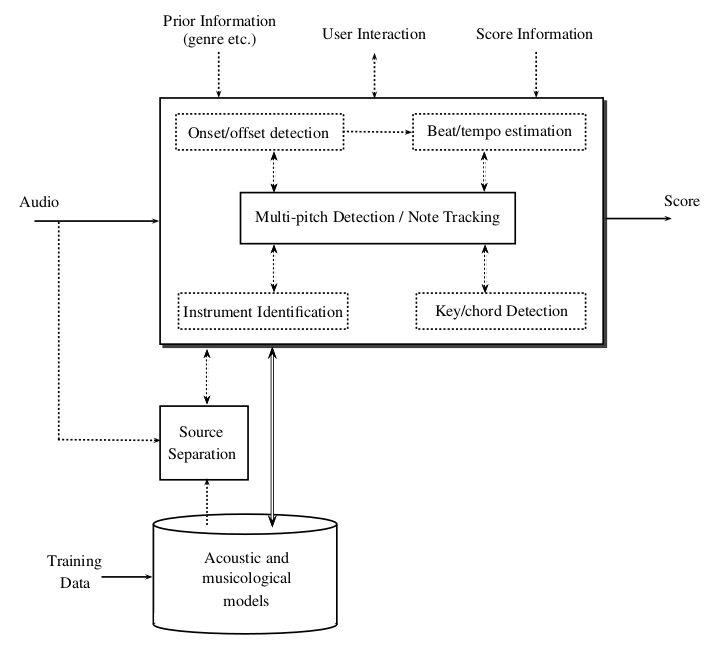
\includegraphics[height=95mm, width=130mm]{z_images/1_contexte/1_general_process.png}
	\caption{Transcription automatique <dam>remettre ici la citation de la capture d'écran avec la page</dam>}
	\label{AMT_presentation}
	\textit{Les sous-systèmes et algorithmes optionnels sont présentés à l’aide
    de lignes pointillées. Les doubles flèches mettent en évidence les
connexions entre les systèmes qui incluent la fusion d’informations et une
communication plus interactive entre les systèmes.}
\end{figure}%\newpage

En ADT \cite{Review_ADT}, plusieurs stratégies de répartition
pré/post-processing sont possibles pour la détection multi-pitchs. Entamer la
détection dès le pré-processing, en supprimant les features non-pertinentes
pendant la séparation des sources afin d’obtenir une meilleure détection des
instruments de la batterie, est une démarche intuitive : supprimer la structure
harmonique pour atténuer l’influence des instruments à hauteurs \florent{haute
fréquence, aigus ?} sur la détection grosse-caisse et caisse-claire en est un
exemple. 
Mais certaines études montrent que des expériences similaires ont donné des
résultats non-concluants et que la suppression des instruments à hauteurs peut
avoir des effets néfastes sur les performances de l’ADT. En outre, les systèmes
d’ADT basés sur des réseaux de neurones récurrents (RNN) ou sur des
factorisations matricielles non négative font la séparation des sources pendant
l’optimisation, ce qui réduit la nécessité de la faire pendant le
pré-processing.

Pour la reconnaissance des instruments, une approche possible \cite{Eronen} 
est de mettre un modèle probabiliste dans l’étape de la classification des
évènements \florent{classification des évènements? la phrase semble redondante}
afin de classer les différents sons de la batterie. Cette méthode permet de se
passer de samples audio isolés en modélisant la progression temporelle des
\textit{features}\footnote{Features : caractéristiques individuelles mesurables
d'un phénomène dans le domaine de l'apprentissage automatique et de la
reconnaissance des formes} avec un modèle de markow caché (HMM). Les
\textit{features} sont transformés en représentations statistiques
indépendantes. \florent{pas clair... peut–être juste mentionner les modèles
probabilistes utilisés} L’approche AdaMa \cite{adama_1} est une autre approche
de la même catégorie ; elle commence par une estimation initiale des sons de la
batterie qui sont itérativement raffinés pour correspondre à (pour matcher)
l’enregistrement visé.
%- Extraction of rhythmic information (tempo, beat, and musical timing)\\

\section{MIDI vers partition}
\florent{ce n'est pas exactement cela. cf. proposition de description + détaillée en commentaires}
%florent:
% Les approches mentionnées en section 2.3 produisent en sortie un fichier MIDI non-quantifié, 
% qui est un format encore très éloigné d'une partition musicale.
% Un premier problème concerne les timings (dates et durées d'événements) qui doivent être alignées
% à des positions temporelles correspondant à des valeurs exprimables avec la notation musicale 
% (cf. la différence performnce vs musique écrite en 1.4)
% On parle de quantification rhythmique.
% Nakamura et al. 2016 présentent une approche de quantification rhythmique avec modèles probba (HMM)
% qui prend en entrée un fichier MIDI non quantifié et fourni en sortie un fichier MIDI quantifié.
% \cite{SHIBATA2021262} étendent ensuite l'approche à une transcription d'enregistrement audio 
% vers un fichier MIDI quantifié.
% Ce dernier format, linéaire, ne correspond toutefois pas encore à une partition structurée, 
% avec groupement rhytmiques hérarchiques, cf. section 1.4.
% dans ces travaux, la structuration des données en npartition est déléguée à un néditeur de 
% partitions MuseScore, avec des résultats assez inégaux.
Le plus souvent, lorsque les articles abordent la transcription automatique de
bout en bout (de l’audio à la partition), l’appellation « \textit{score} »
(partition) désigne un ouput au format Music XML, ou simplement MIDI. 
Par exemple, dans \cite{SHIBATA2021262}, la chaîne de traitement va jusqu’à la
génération d’une séquence MIDI quantifiée qui est importée dans MuseScore pour
en extraire manuellement un fichier MusicXML contenant plusieurs voix.

Seuls quelques travaux récents s’intéressent de près à la création d’outils permettant la génération de partition. 
Le problème de la conversion d'une séquence d'évènements musicaux symboliques 
en une partition musicale structurée est traité notamment dans \cite{foscarin:hal-01988990}. 
Ce travail, qui vise à résoudre en une fois \florent{de manière conjointe}
la quantification rythmique et la production de partition structurée, 
s’appuie tout au long du processus sur des grammaires génératives qui fournissent un modèle hiérarchique 
\florent{langage a priori}
\textit{a priori} des partitions. 
Les expériences ont des résultats prometteurs, mais il faut relever qu’elle ont été menées avec un ensemble de données composé d'extraits monophoniques ; 
il reste donc à traiter le passage au polyphonique, 
\florent{qui nécessite de traiter le problème supplémentaire de la séparation de voix.
i.e. pour la batterie on nveut quantification + structuration + séparation mais seules les 2 premières sont 
couplées dans l'approche de tonn stage.}
en couplant le problème de la séparation des voix avec la quantification du rythme.

L'approche de \cite{foscarin:hal-01988990} est fondée sur la conviction 
que la complexité de la structure musicale dépasse les modèles linéaires.

\section{Approche linéaire et approche hiérarchique}
Plusieurs travaux ont d’abord privilégié l’approche stochastique. Par exemple, Shibata \textit{et al.} \cite{SHIBATA2021262} ont utilisé le modèle de Markov caché (HMM)\footnote{\url{https://fr.wikipedia.org/wiki/Modèle_de_Markov_caché}\\\url{https://en.wikipedia.org/wiki/Hidden_Markov_model}} pour la reconnaissance de la métrique. Les auteurs utilisent d’abord deux réseaux de neurones profonds, l’un pour la reconnaissance des pitchs et l’autre pour la reconnaissance de la vélocité. 
Pour la dernière couche, la probabilité est obtenue par une fonction sigmoïde. Ils construisent ensuite plusieurs HMM métriques étendus pour la musique polyphonique correspondant à des métriques possibles, puis ils calculent la probalitité maximale pour chaque modèle afin d’obtenir la métrique la plus probable.\newpage

\begin{figure}[h]
	\centering
	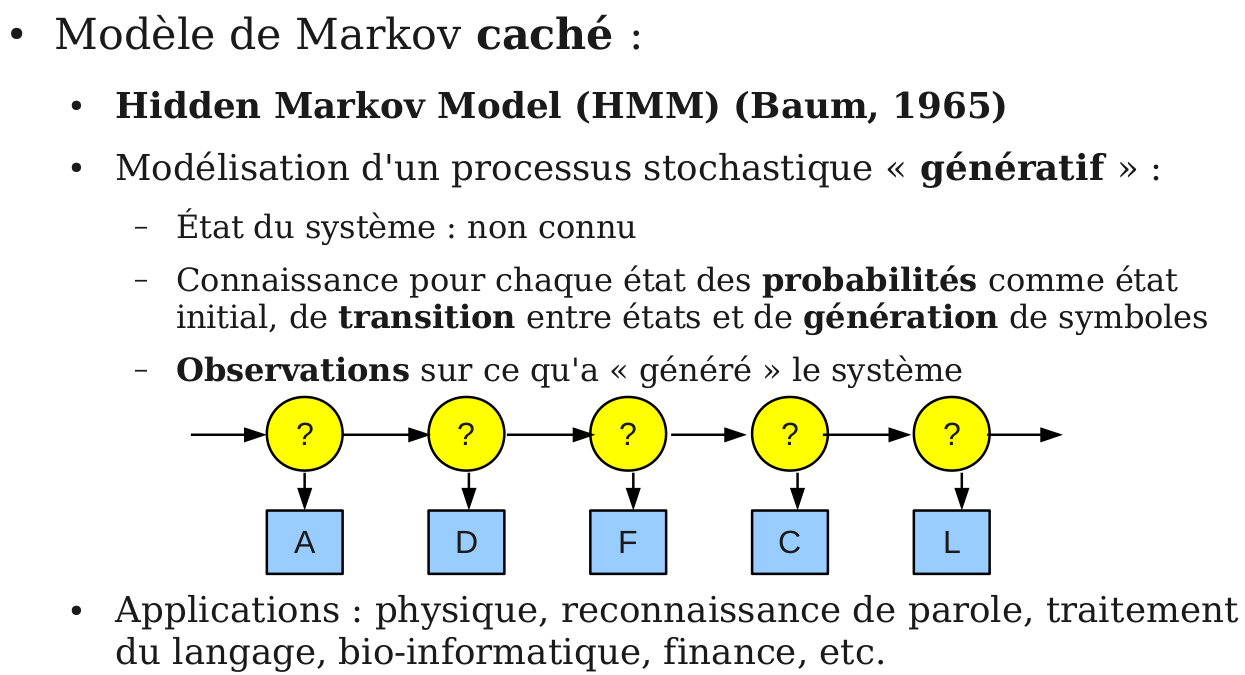
\includegraphics[height=50mm, width=90mm]{z_images/2_etat_de_l_art/0_hmm.png}
	\caption{HMM}
\end{figure}
\textit{Source : Cours de Damien Nouvel\footnote{\url{https://damien.nouvels.net/fr/enseignement}}}\\\\

L’évaluation finale des résultats de \cite{SHIBATA2021262} montre qu’il faut rediriger l’attention vers les valeurs des notes, la séparation des voix et d'autres éléments délicats de la partition musicale qui sont significatifs pour l'exécution de la musique. 
Or, même si la quantification du rythme se fait le plus souvent par la manipulation de données linéaires allant notamment des \textit{real time units} (secondes) vers les musical \textit{time units} (temps, métrique,…), de nombreux travaux suggèrent d’utiliser une approche hiérarchique puisque le langage musical est lui-même structuré.
%
\florent{je ne comprend pas bien l'explication. le pb est plutot vue locale 
(déduction de la proba d'une durée à partir de la durée précédente, par ex. dans un HMM) 
vs vue globale, dans une hiérarchie}
%
En effet, l’usage d’arbres syntaxiques est idéale pour représenter le langage musical. 
Une méthodologie simple pour la description et l'affichage des structures musicales est présentée dans \cite{rythm_tree}. 
Les RT \florent{RT?}
y sont évoqués comme permettant une cohésion complète de la notation musicale traditionnelle avec des notations plus complexes. Jacquemard \textit{et al.} 
\cite{jacquemard:hal-01134096} propose aussi une représentation formelle du rythme, 
inspirée de modèles théoriques antérieurs issus du domaine de la réécriture de termes. 
\florent{techniques de réécriture: appliquée à la déduction automatique, calcul symbolique}
Ils démontrent aussi l’application des arbres de rythmes pour 
\florent{le calcul d'équiv.}
les équivalences rythmiques dans \cite{jacquemard:hal-01403982}. 
La réécriture d’arbres, dans un contexte de composition assistée par ordinateur, 
par exemple, pourrait permettre de suggérer à un utilisateur diverses notations possibles pour une valeur rythmique, avec des complexités différentes.

La nécessité d’une approche hiérarchique pour la production automatique de partition est évoquée dans \cite{foscarin:hal-01988990}. 
\florent{citer thèse de David Rizo (Valencia)}
Les modèles de grammaire qui y sont exposés sont différents de modèles markoviens linéaires de précédents travaux.\newpage
\begin{figure}[h]
	\centering
	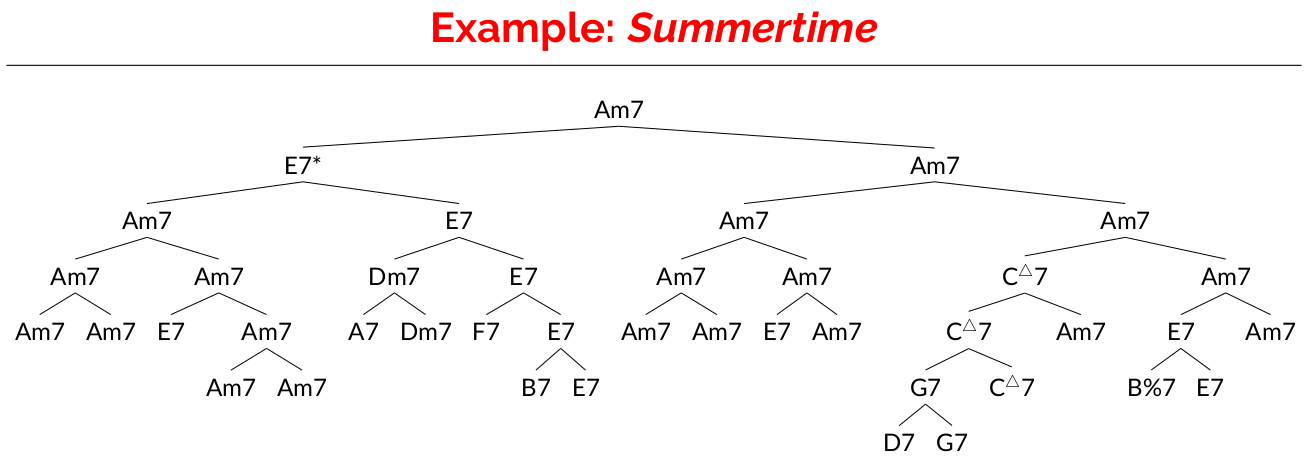
\includegraphics[height=40mm, width=120mm]{z_images/2_etat_de_l_art/1_summertime_tree.png}
	\caption{arbre\_jazz}
	\textit{Représentation arborescente d’une grille harmonique} \cite{harasimjazz}
\end{figure}

\section*{Conclusion}
La plupart des travaux déjà existants sur l’ADT ont été énumérés par Wu \textit{et al.} \cite{Review_ADT} qui, 
pour mieux comprendre la pratique des systèmes d’ADT, se concentrent sur les méthodes basées sur la factorisation matricielle non négative et celles utilisant des réseaux neuronaux récurrents. 
La majorité de ces recherches se concentre sur des méthodes de calcul pour la détection d'événements sonores de batterie à partir de signaux acoustiques ou sur la séparation entre les évènements sonores de batterie avec ceux des autres instruments dans un orchestre ou un groupe de musique \cite{2802}, ainsi que sur l'extraction de caractéristiques de bas niveau telles que la classe d'instrument et le moment de l'apparition du son. 
Très peu d'entre eux ont abordé la tâche de générer des partitions de batterie et, même quand le sujet est abordé, l’output final n’est souvent qu’un fichier MIDI ou MusicXML et non une partition écrite.
\florent{à ma connaissance, aucun des travaux en nADT ne produit de partition XML}

\florent{diff. pour production de partition (et 1 des obj. du stage) est...}
Il n’existe pas de formalisation de la notation de la batterie ni de réelle génération de partition finale, 
dont les enjeux principaux seraient :\\1) le passage du monophonique au polyphonique, comprenant la distinction entre les sons simultanés et les flas ou autres ornements ;\\2) les choix d’écritures spécifiques à la batterie concernant la séparation des voix et les continuations.
\florent{latex: enumerate}
